\documentclass[notheorems,mathserif,table,compress]{beamer}  %dvipdfm选项是关键,否则编译统统通不过
%%------------------------常用宏包------------------------
%%注意, beamer 会默认使用下列宏包: amsthm, graphicx, hyperref, color, xcolor, 等等
\usepackage{fontspec,xunicode,xltxtra}  % for XeTeX
\usepackage{graphicx}
\usepackage{fancybox}
\usepackage{comment}
\usepackage{booktabs}
%%------------------------ThemeColorFont------------------------
%% Presentation Themes
% \usetheme[<options>]{<name list>}
\usetheme{Madrid}
%% Inner Themes
% \useinnertheme[<options>]{<name>}
%% Outer Themes
% \useoutertheme[<options>]{<name>}
\useoutertheme{miniframes} 
%% Color Themes 
% \usecolortheme[<options>]{<name list>}
%% Font Themes
% \usefonttheme[<options>]{<name>}
\setbeamertemplate{background canvas}[vertical shading][bottom=white,top=structure.fg!7] %%背景色, 上25%的蓝, 过渡到下白.
\setbeamertemplate{theorems}[numbered]
\setbeamertemplate{navigation symbols}{}   %% 去掉页面下方默认的导航条.

\usepackage{zhfontcfg}
\usepackage{subfigure}
\usepackage{pgf}
\usepackage{color}
\usepackage{caption}

%\setsansfont[Mapping=tex-text]{文泉驿正黑}  %% 需要fontspec宏包
     %如果装了Adobe Acrobat,可在font.conf中配置Adobe字体的路径以使用其中文字体
     %也可直接使用系统中的中文字体如SimSun,SimHei,微软雅黑 等
     %原来beamer用的字体是sans family;注意Mapping的大小写,不能写错
     %设置字体时也可以直接用字体名,以下三种方式等同:
     %\setromanfont[BoldFont={黑体}]{宋体}
     %\setromanfont[BoldFont={SimHei}]{SimSun}
     %\setromanfont[BoldFont={"[simhei.ttf]"}]{"[simsun.ttc]"}
%%------------------------MISC------------------------
\graphicspath{{figures/}}         %% 图片路径. 本文的图片都放在这个文件夹里了.
%%------------------------正文------------------------
%\pgfputat{\pgfxy(3,-6)}{\pgfbox[centering,base]{\includegraphics[width=2cm,height=2cm]{figures/ouc}}}
\begin{document}

\XeTeXlinebreaklocale "zh"         % 表示用中文的断行
\XeTeXlinebreakskip = 0pt plus 1pt % 多一点调整的空间
%%----------------------------------------------------------
%% This is only inserted into the PDF information catalog. Can be left
%% out.
%%%
%% Delete this, if you do not want the table of contents to pop up at
%% the beginning of each subsection:
\AtBeginSection[]{                              % 在每个Section前都会加入的Frame
  \frame<handout:0>{
    \frametitle{下一节内容}\small
    \tableofcontents[current,currentsubsection]
  }
}
\AtBeginSubsection[]                            % 在每个子段落之前
{
  \frame<handout:0>                             % handout:0 表示只在手稿中出现
  {
    \frametitle{下一节内容}\small
    \tableofcontents[current,currentsubsection] % 显示在目录中加亮的当前章节
  }
}
%%----------------------------------------------------------
\title{图像中环结构特征及其应用}

 \author[孙雪]{\hspace{-2em}学生~~\textcolor{olive}{孙~~~雪}\\
                             \hspace{-2em}导师~~\textcolor{olive}{郑海永}\\
                             \hspace{-2em}\hspace{4em}专业~~信号与信息处理}
    \institute[中国海洋大学]{\kai \textcolor{violet}{中国海洋大学~~信息科学与工程学院}}
%\author[孙雪]{{孙~~~雪}\\
%{指导老师~郑海永}}
%\institute[中国海洋大学]{\small\textcolor{violet}{\textsf{中国海洋大学}}}
\date{2015年5月}
\titlegraphic{
\includegraphics[height=2cm]{ouc}}
%\begin{figure}
%\centering
%    \includegraphics[width=4cm]{figures/ouc}\medskip
%\end{figure}
%\titlegraphic{\vspace{-6em}\includegraphics[height=7cm]{ouc}\vspace{-6em}}
\frame{ \titlepage }
%%----------------------------------------------------------
%\section*{Content}
\frame{\frametitle{内容提要}\tableofcontents}
%%----------------------------------------------------------
\small
\newcommand{\shadow}[2][blue]{\hskip5pt\shadowbox{\color{#1}\Huge #2\vspace{3mm}}}

\section{课题背景}

\begin{frame}
\frametitle{课题背景}
\begin{itemize}
\item {\color{red}{局部特征}}可减小算法的复杂度,提高有效性。
\item {\color{red}{环结构特征}}由图像中存在的交叉、分叉点及它们的连线组成。
\item 应用于图像识别、图像配准等各个领域。
\end{itemize}
\begin{figure}[H]
\centering
  \begin{minipage}[b]{0.33\textwidth} 
      \centering 
      \includegraphics[width=3cm]{chap02/building}
    \end{minipage}
  \begin{minipage}[b]{0.33\textwidth}
    \centering
    \includegraphics[width=3cm]{chap02/reaf}
  \end{minipage}
  \begin{minipage}[b]{0.33\textwidth}
    \centering
    \includegraphics[width=3cm]{chap02/retinal}
  \end{minipage}
  \begin{minipage}[b]{0.33\textwidth}
    \centering
    \includegraphics[width=3cm]{chap02/scallop}
  \end{minipage}
\caption*{\color{blue}{图像中的环结构}}
\end{figure}
\end{frame}

\section{环结构特征}
\begin{frame}
\frametitle{整体框架}
\begin{figure}
\centering
    \centering
    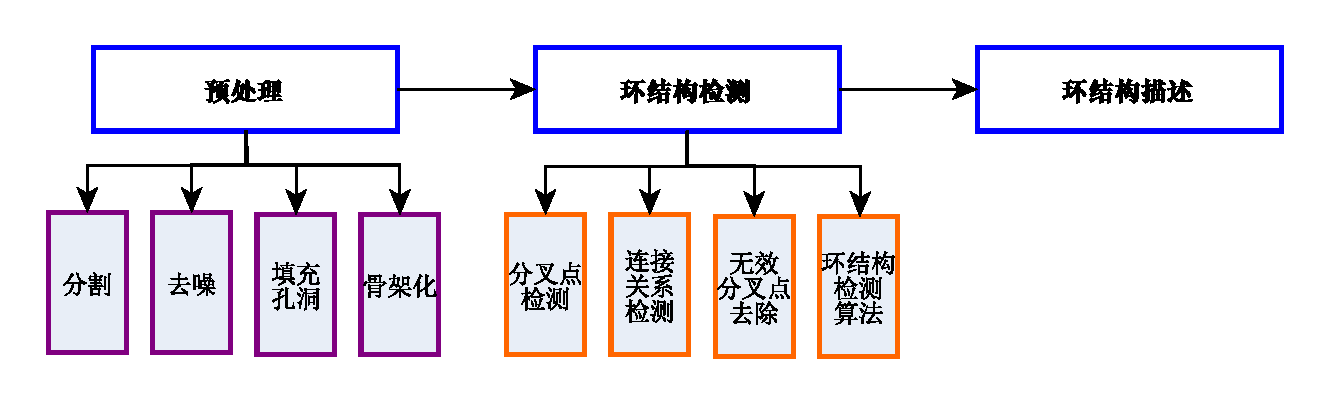
\includegraphics[width=12cm]{chap02/cycle-framework}\medskip
\end{figure}
\end{frame}

\begin{frame}
\frametitle{整体框架}
\begin{figure}
\centering
    \centering
    \includegraphics[width=12cm]{chap02/cycle-framework1}\medskip
\end{figure}
\end{frame}

\begin{frame}
\frametitle{预处理}
\begin{figure}
\centering
    \centering
    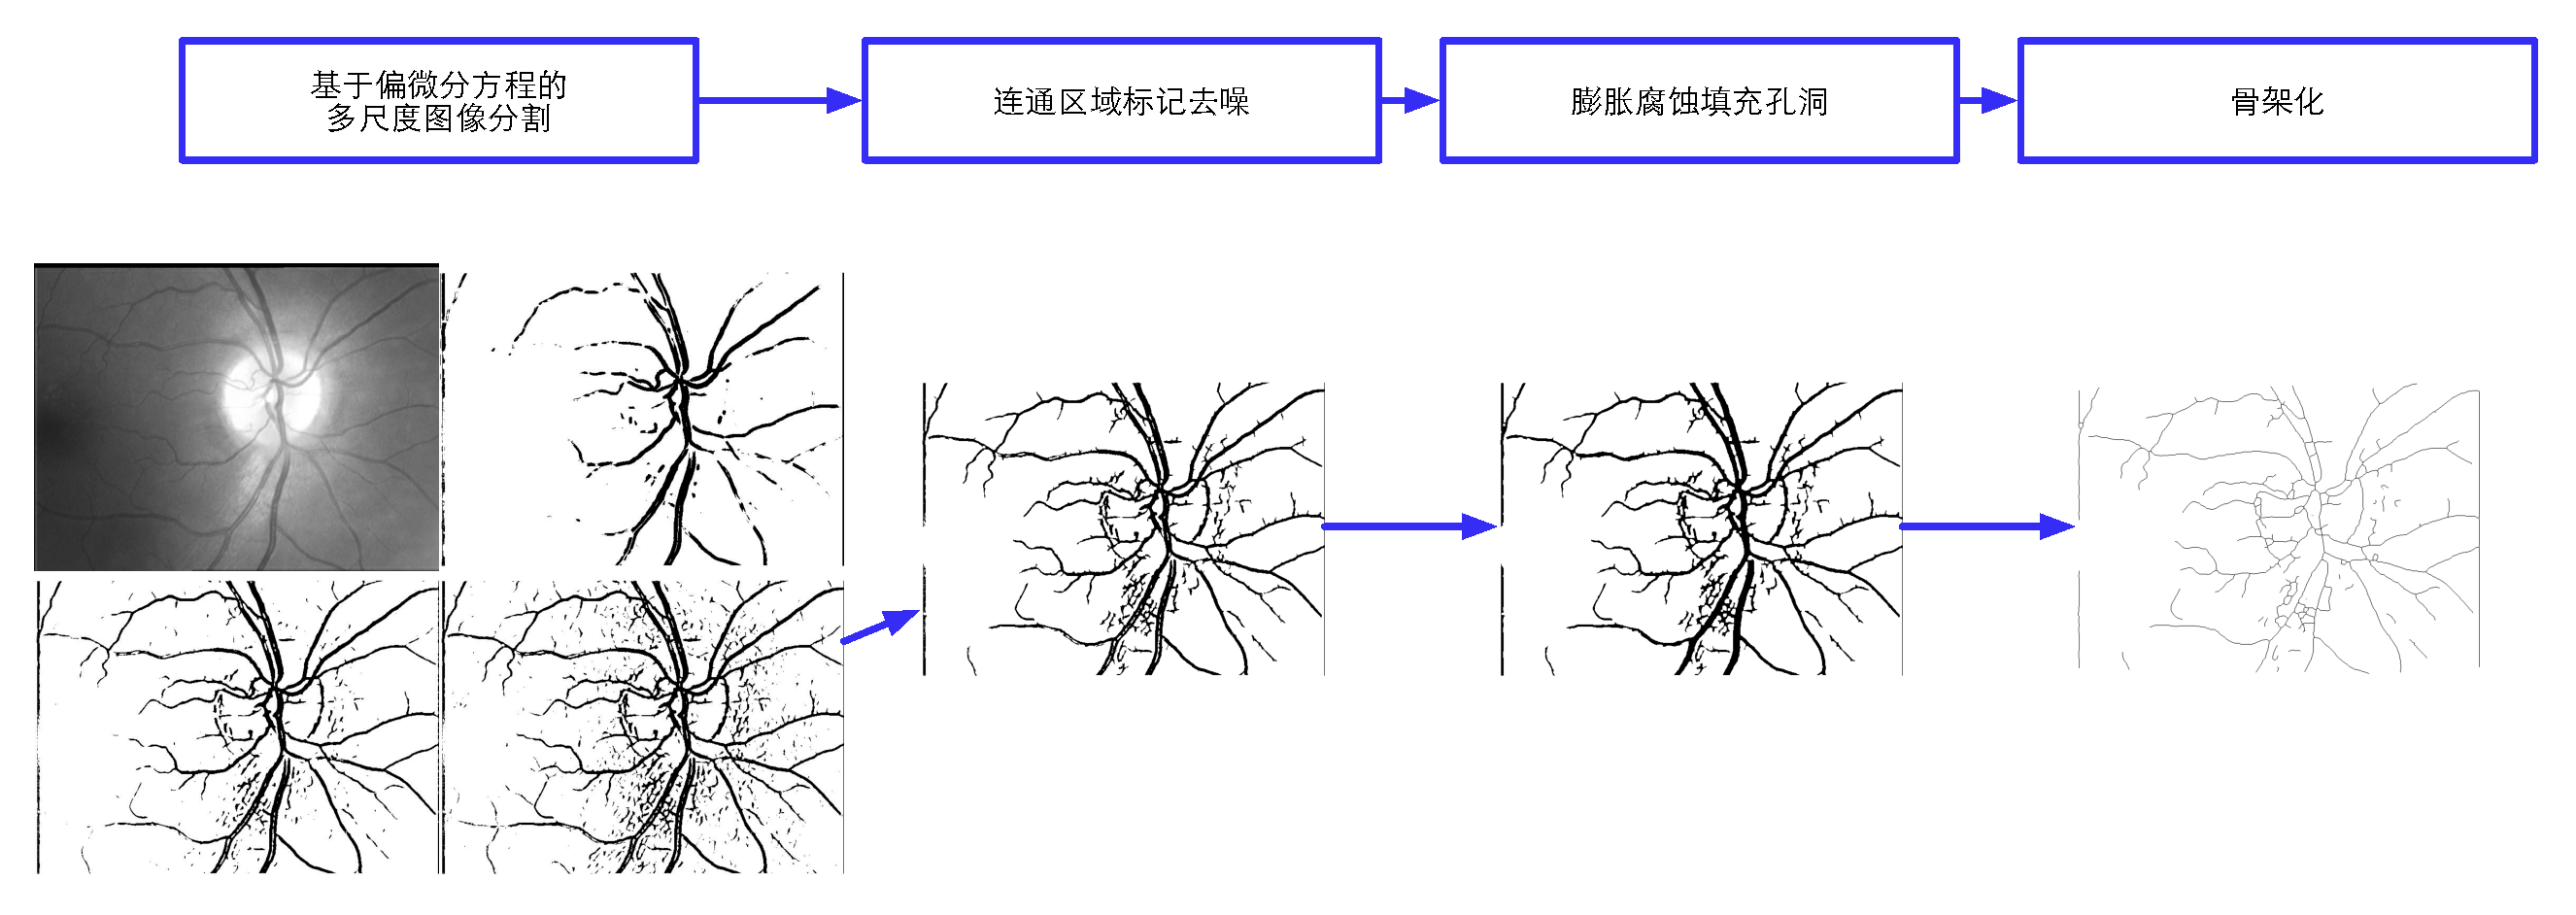
\includegraphics[width=12.5cm]{chap02/processing}\medskip
\end{figure}
\end{frame}

\begin{frame}
\frametitle{整体框架}
\begin{figure}
    \centering
    \includegraphics[width=12cm]{chap02/cycle-framework2}\medskip
\end{figure}
\end{frame}

\begin{frame}
\frametitle{图像{\color{white}{$\Rightarrow$}}图}

\begin{figure}
\centering
    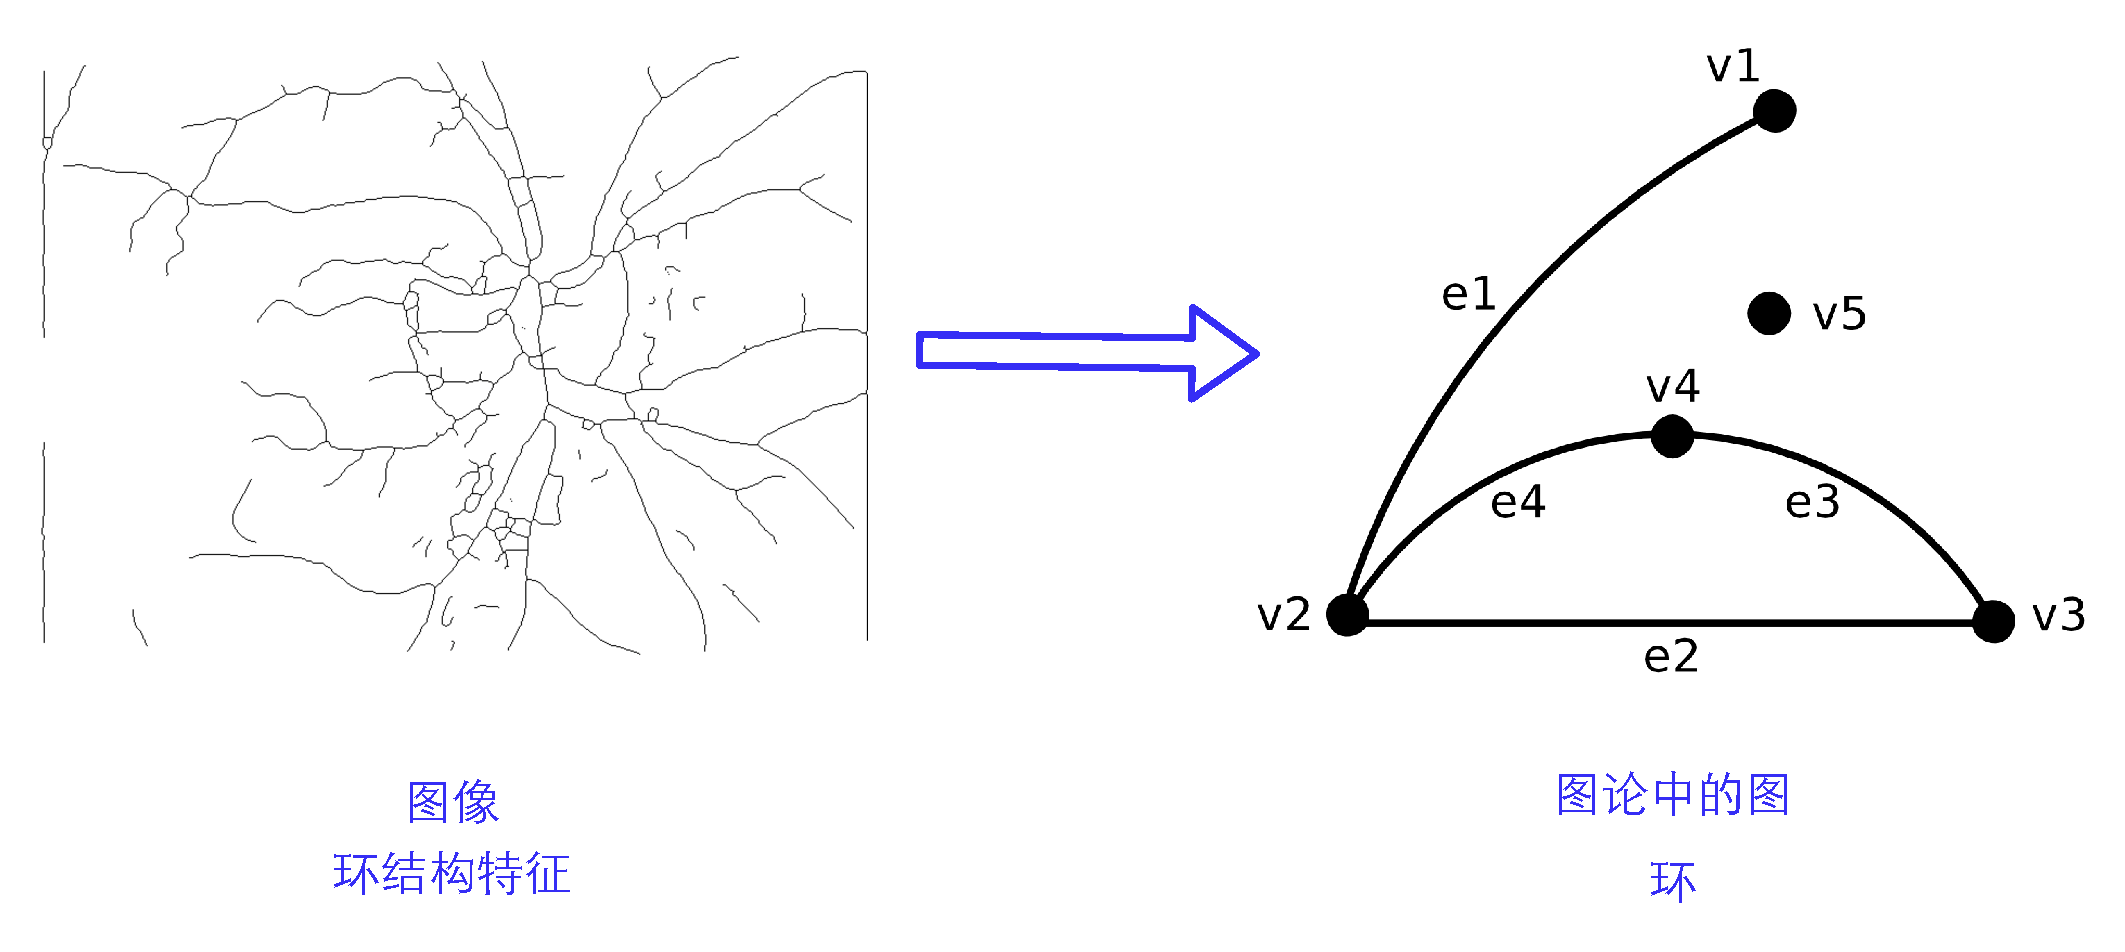
\includegraphics[width=10cm]{chap02/image-graph}\medskip
\end{figure}
\end{frame}



\begin{frame}
\frametitle{1. 图像中的分叉点检测}
\begin{enumerate}
\item 检测图像中的线(假设背景为黑,线为白,即背景像素值为$0$,线为$1$)
\item 以每个线上的点为对象,检测其八邻域像素值
\item 若八邻域少于$3$个像素值为$1$,则不认为是分叉点。
\item 若八邻域有$3$个像素值为$1$,则认为是三分叉点。
\item 若八邻域多于$3$个像素为$1$,则把中心像素作为分叉点。
\end{enumerate}
\begin{figure}
\centering
  \begin{minipage}[b]{0.33\textwidth} 
      \centering 
      \includegraphics[width=3cm]{chap02/3FeaturePoint}
    \end{minipage}
  \begin{minipage}[b]{0.33\textwidth}
    \centering
    \includegraphics[width=3cm]{chap02/4FeaturePoint}
  \end{minipage}
\caption*{\color{blue}{三分叉点与四分叉点}}
\end{figure}
\end{frame}

\begin{frame}
\frametitle{2. 连接关系检测}
\begin{enumerate}
\item 每个分叉点被看做一个种子。
\item 沿种子点八邻域像素值为$1$的方向不断向外扩展,直到找到与种子点相邻的分叉点。
\item 遍历所有分叉点后,所有的分叉点及其连接关系被检测到。
\end{enumerate}
\begin{figure}
\begin{minipage}[b]{0.48\textwidth} 
      \centering 
      \includegraphics[width=4cm]{chap02/graph}
\caption*{\color{blue}{图}}
    \end{minipage}
\begin{minipage}[b]{0.48\textwidth} 
\begin{tabular}{p{1.2cm}<{\centering}p{0.5cm}<{\centering}p{0.5cm}<{\centering}p{0.5cm}<{\centering}}
  \hline
  分叉点 & \multicolumn{3}{c}{相邻分叉点}\\
  \hline
  \rowcolor{gray!50}
  $v_{1}$ & $v_{2}$  & $0$      & $0$  \\
  $v_{2}$ & $v_{1}$  & $v_{3}$  & $v_{4}$ \\
  \rowcolor{gray!50}
  $v_{3}$ & $v_{2}$  & $v_{4}$  & $0$\\
  $v_{4}$ & $v_{2}$  & $v_{3}$  & $0$ \\
  \rowcolor{gray!50}
  $v_{5}$ & $0$      & $0$      & $0$\\
  \hline
\end{tabular}
\caption*{\color{blue}{点---边关系}}
\end{minipage}
\end{figure}
\end{frame}

\begin{frame}
\frametitle{3. 滤除无效分叉点}
\begin{block}<+->{条件}
\begin{itemize}
\item 每个分叉点的度大于3\\
\item 在点---边关系中出现3次以上
\end{itemize}
\end{block}
\begin{figure}
\centering
  \begin{minipage}[b]{0.33\textwidth} 
      \centering 
      \includegraphics[width=3.5cm]{chap02/all-bifu}
    \end{minipage}
  \begin{minipage}[b]{0.33\textwidth}
    \centering
    \includegraphics[width=3.5cm]{chap02/select-bifu}
  \end{minipage}
\caption*{\color{blue}{所有分叉点与滤除无效分叉点后的对比图}}
\end{figure}
\end{frame}

\begin{frame}
\frametitle{4. 基于广度优先策略的环结构检测}
\begin{figure}
\centering
  \begin{minipage}[b]{0.48\textwidth} 
      \centering 
       \includegraphics[width=5cm]{chap02/graph2}
    \end{minipage}
  \begin{minipage}[b]{0.48\textwidth}
    \centering
    \includegraphics[width=4cm]{chap02/tree}
  \end{minipage}
\caption*{\color{blue}{图与搜索树}}
\end{figure}
\end{frame}

\begin{frame}
\frametitle{整体框架}
\begin{figure}
\centering
    \centering
    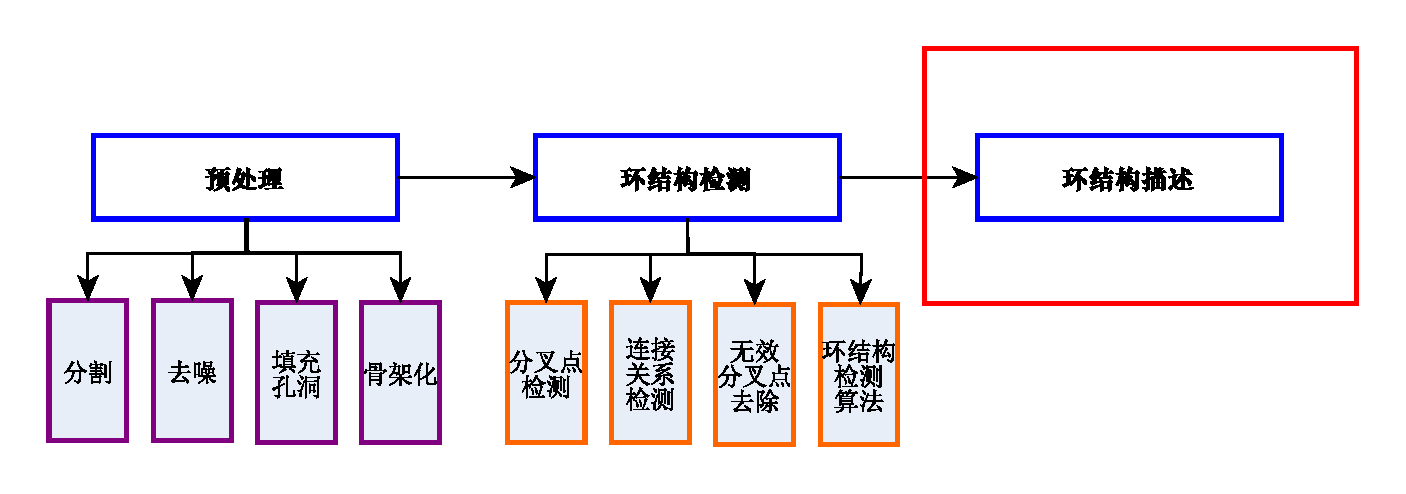
\includegraphics[width=12cm]{chap02/cycle-framework3}\medskip
\end{figure}
\end{frame}

\begin{frame}
\frametitle{环结构描述}
\begin{figure}[H]
\centering
\includegraphics[width=0.4\textwidth]{chap02/description.pdf}
\caption*{\color{blue}{环结构描述}}
\end{figure}
\begin{multline}
\tilde{v}=\{\textrm{长度,角度}\}=\{L_{1},L_{2},L_{3},L_{4},\theta_{1},\theta_{2},\theta_{3},\mathbf{0},\theta_{4},\\\theta_{5},\theta_{6},\theta_{7},\theta_{8},\theta_{9},\theta_{10},\theta_{11},\theta_{12},\theta_{13},\theta_{14},\mathbf{0},\theta_{15},\theta_{16},\theta_{17},\theta_{18}\}
\end{multline}
\begin{center}
\color{red} \fbox{环结构特征具有平移、旋转、缩放不变性}
\end{center}
\end{frame}
\section{环结构特征在视网膜图像配准中的应用}

\begin{frame}
\frametitle{基本框架}
\begin{figure}
  \centering
  \includegraphics[width=1\textwidth]{chap03/framework}
  \caption*{\color{blue}{基本框架}}
\end{figure}
\end{frame}

\begin{frame}
\frametitle{1. 相似性度量}
\begin{itemize}
\item 欧式距离:
\begin{equation}
d_{12}=\sqrt{(x_1-x_2)^2+(y_1-y_2)^2}
\end{equation}
\begin{align}
D_{pq} = \sqrt{(|V_p-W_q|)^2}, p = 1, 2, \ldots, m; q = 1, 2, \ldots, n
\end{align}
\item 曼哈顿距离:
\begin{equation}
d_{12}=|x_1-x_2|+|y_1-y_2| 
\end{equation}
\begin{align}
D_{pq} = mean(|V_p-W_q|), p = 1, 2, \ldots, m; q = 1, 2, \ldots, n
\end{align}
\begin{center}
\color{red} \fbox{曼哈顿距离比欧式距离更适合做环结构特征的相似性度量}
\end{center}
\end{itemize}
\end{frame}

%\begin{frame}
%\frametitle{相似性度量结果}
%\begin{figure}
%  \begin{minipage}[b]{0.48\textwidth}
%    \centering
%    \includegraphics[width=3.5cm]{chap03/bw1-all-cycles}
%     \caption*{\color{blue}{参考图像中所有环结构}}
%  \end{minipage}
%  \begin{minipage}[b]{0.48\textwidth}
%    \centering
%    \includegraphics[width=3.5cm]{chap03/bw2-all-cycles}
%     \caption*{\color{blue}{待配准图像中所有的环结构}}
%  \end{minipage}
% \begin{minipage}[b]{0.48\textwidth}
%    \centering
%      \includegraphics[width=3.5cm]{chap03/bw1-matching-cycles}
%     \caption*{\color{blue}{参考图像中最匹配的环结构}}
 %   \end{minipage}
%\begin{minipage}[b]{0.48\textwidth}
%	\centering
%      \includegraphics[width=3.5cm]{chap03/bw2-matching-cycles}
%     \caption*{\color{blue}{待配准图像中最匹配的环结构}}
%    \end{minipage}
%\end{figure}
%\end{frame}

\begin{frame}
\frametitle{2. 相似性变换}
\begin{figure}
\centering
\begin{minipage}[b]{0.48\textwidth} 
      \centering 
      \includegraphics[width=3.5cm]{chap03/R096}
     \caption*{\color{blue}{参考图像}}
\end{minipage}
  \begin{minipage}[b]{0.48\textwidth}
    \centering
    \includegraphics[width=3.5cm]{chap03/R212}
     \caption*{\color{blue}{待配准图像}}
  \end{minipage}
  \begin{minipage}[b]{0.48\textwidth}
    \centering
    \includegraphics[width=3.5cm]{chap03/096-212-result}
     \caption*{\color{blue}{原始配准结果}}
  \end{minipage}
  \begin{minipage}[b]{0.48\textwidth}
    \centering
    \includegraphics[width=3.5cm]{chap03/096-212-local}
          \caption*{\color{blue}{骨架化配准结果}}
  \end{minipage}
\end{figure}
\end{frame}

\begin{frame}
\frametitle{3. 骨架化对准精度}
\begin{enumerate}
\item 计算配准结果中与参考图像中的血管点在一定区域内最近的血管点。
\vspace{0.5cm}
\item 若这个区域中没有与这个血管点相邻最近的点,则标记这个血管点无效。
\vspace{0.5cm}
\item 骨架化对准精度被定义为$SAEM = (\sum d) / Num_v$。

\end{enumerate}
\end{frame}

\begin{frame}
\frametitle{4. 对比实验}
\begin{itemize}
\item VARIA数据库。经过挑选与组合,共得到$153$对图像以做配准。
\vspace{2mm}
\item 不同变换模型之间的对比实验
\vspace{2mm}
\item 不同特征之间的对比实验
\end{itemize}
\end{frame}

\begin{frame}
\frametitle{不同变换模型之间的对比实验}
\begin{figure}
\centering
\begin{minipage}[b]{0.3\textwidth} 
      \centering 
      \includegraphics[width=3cm]{chap03/similarity1.png}
\end{minipage}
\begin{minipage}[b]{0.3\textwidth}
    \centering
    \includegraphics[width=3cm]{chap03/affine1.png}
  \end{minipage}
\begin{minipage}[b]{0.3\textwidth}
	\centering
      \includegraphics[width=3cm]{chap03/polynomial1.png}
    \end{minipage}
\caption*{\color{blue}{相似性变换、仿射变换、二次多项式变换}}
\end{figure}
\begin{table}
\centering
\begin{tabular}{lcc}
\toprule
变换模型 & SR  & SAEM (像素)\\
\midrule
相似性变换 & $\mathbf{96.73\%}$ & $\mathbf{0.938}$ \\
仿射变换 & $50.33\%$ & $1.010$              \\
二次多项式变换 & $16.99\%$ & $0.231$\\
\bottomrule
\end{tabular}
\label{tab:models}
\end{table}
\end{frame}

\begin{frame}
\frametitle{不同特征之间的对比实验}
基于分叉结构的配准方法:
\begin{figure}
  \centering
  \includegraphics[width=0.4\textwidth]{chap03/bifurcation-structure}
  \caption*{\color{blue}{分叉结构特征}}
\end{figure}
\end{frame}

\begin{frame}
\frametitle{不同特征之间的对比实验}
\begin{figure}
\begin{minipage}[b]{0.48\textwidth}
    \centering
    \includegraphics[width=4cm]{chap03/bifu2.png}
  \end{minipage}
\begin{minipage}[b]{0.48\textwidth}
    \centering
    \includegraphics[width=4cm]{chap03/ours2.png}
  \end{minipage}
\caption*{\color{blue}{分叉结构特征与环结构特征}}
\end{figure}

\begin{table}
\centering
\begin{tabular}{lcc}
\toprule
特征 & SR & SAEM (pixel)\\
\midrule
分叉结构 & $52.9\%$ & $1.009$\\
环结构 & $\mathbf{96.73\%}$ & $\mathbf{0.938}$\\
\bottomrule
\end{tabular}
\end{table}

\end{frame}
\section{环结构特征在扇贝图像识别中的应用}

\begin{frame}
\frametitle{整体框图}
\begin{figure}
  \centering
  \includegraphics[width=0.8\textwidth]{chap04/scallop-framework}
\end{figure}
\end{frame}

\begin{frame}
\frametitle{扇贝图像库的构建}
\begin{itemize}
\item 标准图像库。共包含$10$幅不同扇贝个体的图像。
\item 待识别图像库。待识别图像库中的扇贝图像是参考图像库中的图像经过{\color{red}{旋转}}、{\color{red}{缩放}}、{\color{red}{遮挡}}处理得到的,故待识别图像库中共包含$30$幅图像。
\end{itemize}
\begin{figure}
\centering
  \begin{minipage}[b]{0.33\textwidth} 
      \centering 
      \includegraphics[width=3cm]{chap04/28-ori}
    \end{minipage}
  \begin{minipage}[b]{0.33\textwidth}
    \centering
    \includegraphics[width=4cm]{chap04/28-da}
    \end{minipage}
  \begin{minipage}[b]{0.33\textwidth} 
      \centering 
      \includegraphics[width=3cm]{chap04/28-qu}
    \end{minipage}
  \begin{minipage}[b]{0.33\textwidth}
    \centering
    \includegraphics[width=2.5cm]{chap04/28-zhuan}
  \end{minipage}
\caption*{\color{blue}{扇贝参考图像与待识别图像}}
\end{figure}
\end{frame}


\begin{frame}
\frametitle{识别结果}
\begin{figure}
\centering
  \begin{minipage}[b]{0.3\textwidth} 
      \centering 
      \includegraphics[width=2.8cm]{chap04/suoxiao-yuantu}
    \end{minipage}
  \begin{minipage}[b]{0.3\textwidth} 
      \centering 
      \includegraphics[width=2.8cm]{chap04/zhegai-yuantu}
    \end{minipage}
  \begin{minipage}[b]{0.3\textwidth} 
      \centering 
      \includegraphics[width=2.8cm]{chap04/xuanzhuan-yuantu}
    \end{minipage}

  \begin{minipage}[b]{0.3\textwidth}
    \centering
    \includegraphics[width=2.8cm]{chap04/suoxiao}
    \end{minipage}
  \begin{minipage}[b]{0.3\textwidth}
    \centering
    \includegraphics[width=2.8cm]{chap04/zhegai}
    \end{minipage}
  \begin{minipage}[b]{0.3\textwidth}
    \centering
    \includegraphics[width=2.8cm]{chap04/xuanzhuan}
    \end{minipage}
\caption*{\color{blue}{扇贝参考图像与待识别图像中匹配的环结构}}
\end{figure}
\begin{center}
\color{red} \fbox{$30$幅图像的最终识别结果为$83.3\%$}
\end{center}
\end{frame}


\section{总结与展望}
\begin{frame}
\frametitle{总结}
\begin{itemize}
\item 环结构特征提取与描述
\vspace{2mm}
\item 基于环结构特征的视网膜图像配准
\vspace{2mm}
\item 基于环结构特征的扇贝图像识别
\end{itemize}
\end{frame}

\begin{frame}
\frametitle{展望}
\begin{itemize}
\item 环结构检测算法的通用性
\vspace{2mm}
\item 图像分割的最优尺度的选择
\vspace{2mm}
\item 角毛藻图像的识别
\end{itemize}
\end{frame}

\begin{frame}
\begin{center}
\huge\shadow{\textit{请各位老师批评指正!}}
\end{center}
\end{frame}

\end{document}
